\documentclass[tikz, border=10pt]{standalone}
\usetikzlibrary{arrows.meta, positioning, calc, fit, backgrounds}

\begin{document}
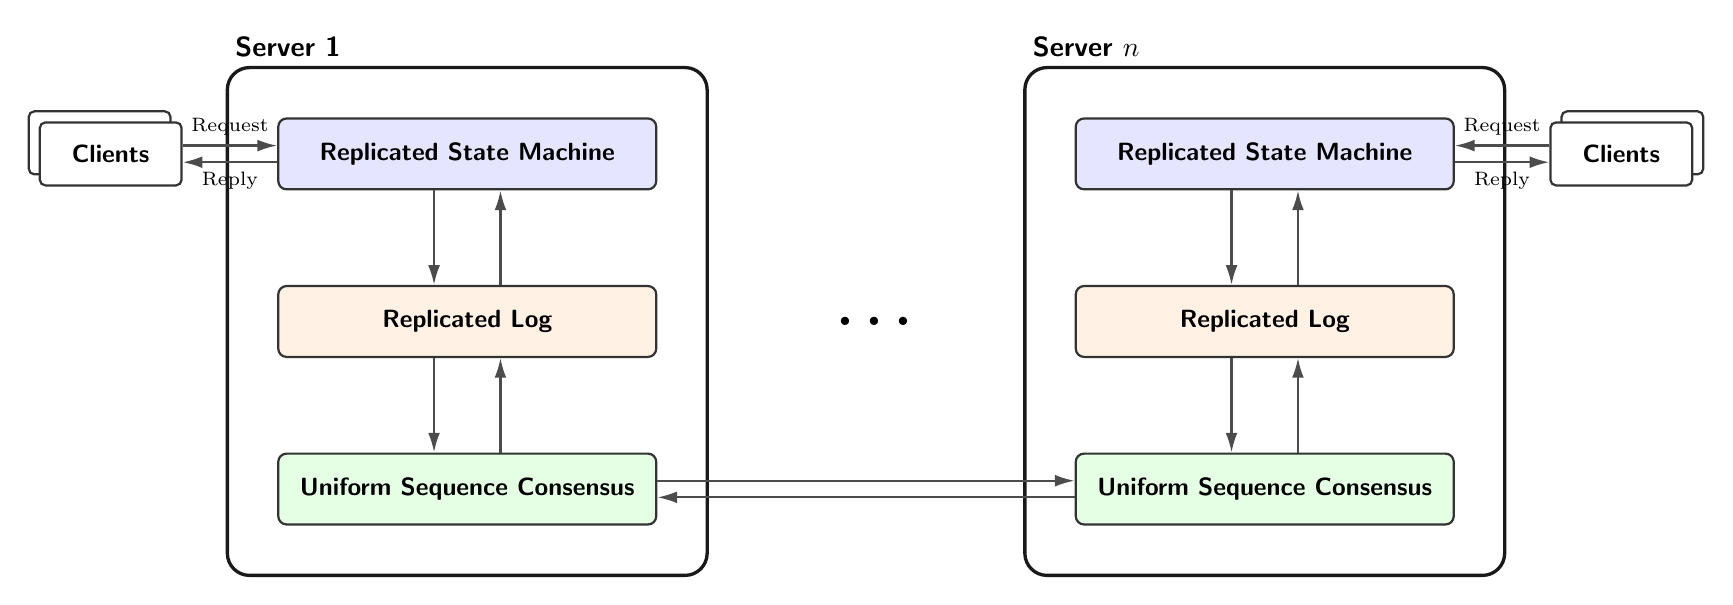
\begin{tikzpicture}[
    font=\sffamily,
    node distance=1.2cm and 2.5cm,
    % Box Styles
    component/.style={
        rectangle, rounded corners=3pt, draw=black!80, thick,
        minimum width=4.8cm, minimum height=0.9cm, align=center, font=\sffamily\small\bfseries
    },
    rsm/.style={component, fill=blue!10},
    log/.style={component, fill=orange!10},
    cons/.style={component, fill=green!10},
    % Client Style
    client/.style={
        rectangle, rounded corners=2pt, draw=black!80, thick,
        fill=white, minimum width=1.8cm, minimum height=0.8cm, font=\sffamily\small\bfseries
    },
    % Frame Style
    serverFrame/.style={
        rectangle, rounded corners=8pt, draw=black!90, very thick, inner sep=18pt
    },
    % Arrow Style
    myArrow/.style={-{Latex[length=2.5mm, width=1.5mm]}, thick, draw=black!70}
]

    % --- SERVER 1 ---
    \node[rsm] (rsm1) {Replicated State Machine};
    \node[log, below=of rsm1] (log1) {Replicated Log};
    \node[cons, below=of log1] (cons1) {Uniform Sequence Consensus};
    
    % Group Server 1
    \node[serverFrame, fit=(rsm1) (cons1)] (frame1) {};
    \node[anchor=south west, font=\sffamily\bfseries] at (frame1.north west) {Server 1};

    % --- DOTS ---
    \node[right=of frame1, xshift=-1cm, font=\huge\bfseries] (dots) {\dots};

    % --- SERVER N ---
    \node[rsm, right=of rsm1, xshift=2.8cm] (rsmN) {Replicated State Machine};
    \node[log, below=of rsmN] (logN) {Replicated Log};
    \node[cons, below=of logN] (consN) {Uniform Sequence Consensus};
    
    % Group Server N
    \node[serverFrame, fit=(rsmN) (consN)] (frameN) {};
    \node[anchor=south west, font=\sffamily\bfseries] at (frameN.north west) {Server $n$};

    % --- CLIENTS ---
    % Left Clients (Stacked)
    \node[client, left=1.2cm of rsm1, xshift=-4pt, yshift=4pt] (cl1b) {};
    \node[client, left=1.2cm of rsm1] (cl1) {Clients};
    
    % Right Clients (Stacked)
    \node[client, right=1.2cm of rsmN, xshift=4pt, yshift=4pt] (clNb) {};
    \node[client, right=1.2cm of rsmN] (clN) {Clients};

    % --- ARROWS ---
    % Up/Down Flow
    \foreach \i in {1, N} {
        \draw[myArrow] ([xshift=-12pt]rsm\i.south) -- ([xshift=-12pt]log\i.north);
        \draw[myArrow] ([xshift=12pt]log\i.north) -- ([xshift=12pt]rsm\i.south);
        \draw[myArrow] ([xshift=-12pt]log\i.south) -- ([xshift=-12pt]cons\i.north);
        \draw[myArrow] ([xshift=12pt]cons\i.north) -- ([xshift=12pt]log\i.south);
    }

    % Interaction Arrows
    \draw[myArrow] ([yshift=3pt]cl1.east) -- node[above, font=\scriptsize] {Request} ([yshift=3pt]rsm1.west);
    \draw[myArrow] ([yshift=-3pt]rsm1.west) -- node[below, font=\scriptsize] {Reply} ([yshift=-3pt]cl1.east);

    \draw[myArrow] ([yshift=3pt]clN.west) -- node[above, font=\scriptsize] {Request} ([yshift=3pt]rsmN.east);
    \draw[myArrow] ([yshift=-3pt]rsmN.east) -- node[below, font=\scriptsize] {Reply} ([yshift=-3pt]clN.west);

    % Inter-Server Consensus
    \draw[myArrow] ([yshift=3pt]cons1.east) -- ([yshift=3pt]consN.west);
    \draw[myArrow] ([yshift=-3pt]consN.west) -- ([yshift=-3pt]cons1.east);

\end{tikzpicture}
\end{document}